\documentclass[]{scrartcl}

%opening
\title{March Madness Analysis}
\author{Biased Estimators: Alexander Van Roijen, Molly Clark, Rocco Bavuso}
\usepackage[margin=1.0in]{geometry}
\usepackage{color}
\usepackage{times}
\usepackage[pdftex]{hyperref}


\setlength{\parindent}{0in}
\setlength{\parskip}{2ex}
\renewcommand{\baselinestretch}{1.0}

\usepackage{graphicx}
\usepackage{caption}
\usepackage{float}


\begin{document}

\maketitle

\begin{abstract}
\begin{center}
	\noindent March Madness is an annual NCAA Division I Basketball tournament. The tournament occurs in the month of March, thereby earning its name. There are 64 teams in the tournament each year, seeded into four regions that each contain 16 teams. This report will look at how far each team makes it into the tournament, based on their regular season data and prior tournament success.
\end{center}
\end{abstract}

\section*{Introduction}
\noindent In this report we work with data that was obtained from kaggle.com. We were interested to see what factors most affect a team's success in the March Madness tournament, so we compare teams to each other for every year that we have data. In doing so, we narrow down our predictors to find the best model of a team's success in the tournament for each year.

\noindent We were motivated to look into this data in part because the tournament is so hard to predict from year to year. We wondered what statistics and data from a team's season and history could be used to estimate how far the team would make it in the tournament. It is not uncommon for there to be many upsets over the course of the tournament, which can throw off any model, so we had to consider this uncertainty when choosing the best model.
\section*{Data Summary}
From Kaggle's website, we downloaded a data set that gave us a look at all Division I teams who did or did not qualify for the March Madness tournament in the past 30 or so years. Each team is assigned a four digit code that is consistent from season to season and data set to data set. This allows us to manipulate and analyze the data across the different files.

We had data that was collected during the regular season and data that was collected during the tournament, but in the long run choose to focus our model on regular season data so as to be able to predict the current season's tournament success if need be.

For the years 1985 to 2003, we have data in regards to the wins and losses of each involved team. For the years 2003 to 2016, we have more in depth data that includes each team's statistics from each game all season and throughout the tournament.

We began by looking at the data that has been collected season to season and follow up by looking at the data from previous tournaments and regional and past seed data to see which factors effect a team's chances of winning games in the tournament.

Because this tournament occurs each year, and because our data spans many years, we also saw it fitting to analyze how well teams had performed in the past when trying to predict their success in the future. The expectations and reputation of a team surely have an impact on how well they perform during the season and tournament, so temporal data about past success was essential to our model.

Throughout this report, let the following be universally true:

{\textbf {Field Goals:}} defined as any shot that is made in the game and is worth 2 points (within the 3 point line, not a free throw)

{\textbf {Three Pointers:}} defined as any shot that is made in the game and is worth 3 points (outside the 3 point line, from any place)

{\textbf {Free Throws:}} defined as any shot that is made in the game and is worth 1 point (shot after being fouled in any form, from the free throw line)

{\textbf {Assist:}} defined as a pass to another player who then immediately scores

{\textbf {Rebound:}} defined as a play in which a player grabs the ball, which bounced off of either the rim or backboard on an attempted shot. For this paper, we include offensive and defensive rebounds

{\textbf {Turnovers:}} defined as any action that results in the loss of basketball. (an action that gives the basketball to the other team not including a failed shot attempt)

{\textbf {Steals:}} defined as a defensive play in which a player steals the basketball from an opposing player

{\textbf {Block:}} defined as a defensive play in which a player deflects an opposing shot attempt before it reaches the basket

{\textbf {Personal Fouls:}} defined as an action that results in either a loss of possession or free throws for the other team
\section*{Pre-Analysis}
We began by looking at our data from a lens that based winning teams against losing teams. This was based on who won and lost each game of each season, so it is important to note that it is likely that teams would fall into both categories on occasion. We hoped to find what factors and variables in a season could predict a team's overall success in the tournament and moving forward.

We already had easy access to data that was parsed based on which team had won and which team had lost, so this seemed like a logical first step. We chose to keep regular season data apart from tournament data because the game play is so different in the tournament. In general, it is expected that the involved teams are among the best in the country, and the games have much higher stakes, so statistics may look different.
\subsection*{Regular Season Data}
In working with the regular season data, we first looked at some larger scale averages, comparing winning teams to losing teams on a very basic level.

We compared the average statistics of winning teams to the average statistics of losing teams and found what many would expect: on average, winning teams perform better in areas that are considered "good" statistics, whereas losing teams have higher rates of "bad" statistics.
\begin{figure}[H]
	\begin{center}
	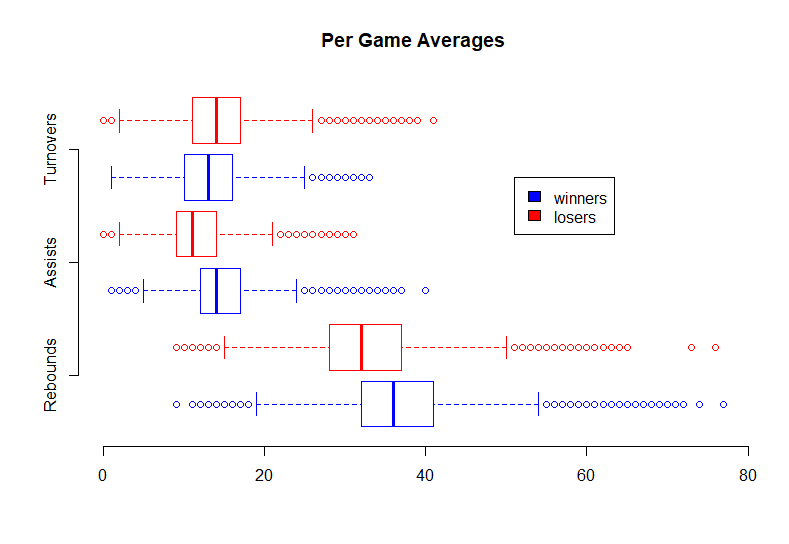
\includegraphics[scale=.4]{GameAverages.png}
	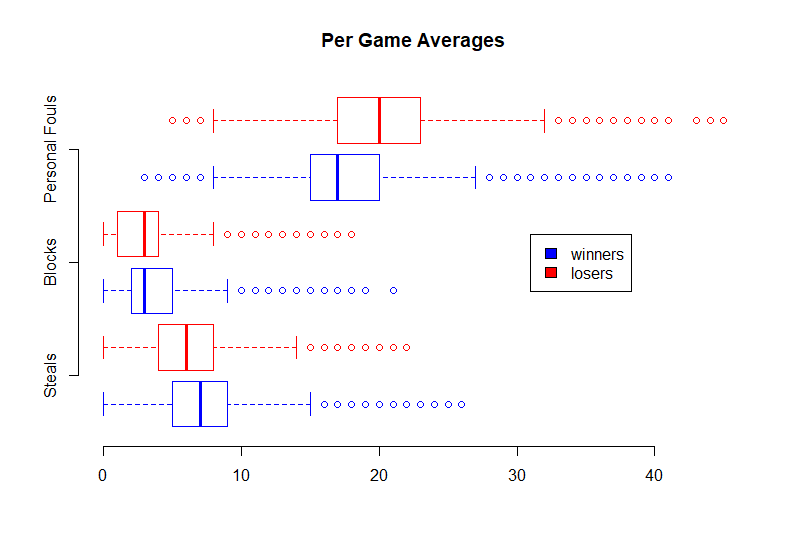
\includegraphics[scale=.4]{GameAverages2.png}
	\end{center}
\end{figure}
The above figures show the distribution of the winning and losing teams' averages throughout the years. They illustrate the above point that winning teams have higher averages in more beneficial statistics such as Rebounds, Assists, and Steals. This is a trend that we take note of when moving forward.

We then looked at winning and losing teams' average shooting percentages for the regular season. We were hoping to find which shots hold the most weight in the game. For example, three point shots are worth more points than any other shots, but free throws offer up an easy opportunity for a point or two and may be necessary late in the game.
\begin{figure}[H]
	\centering
	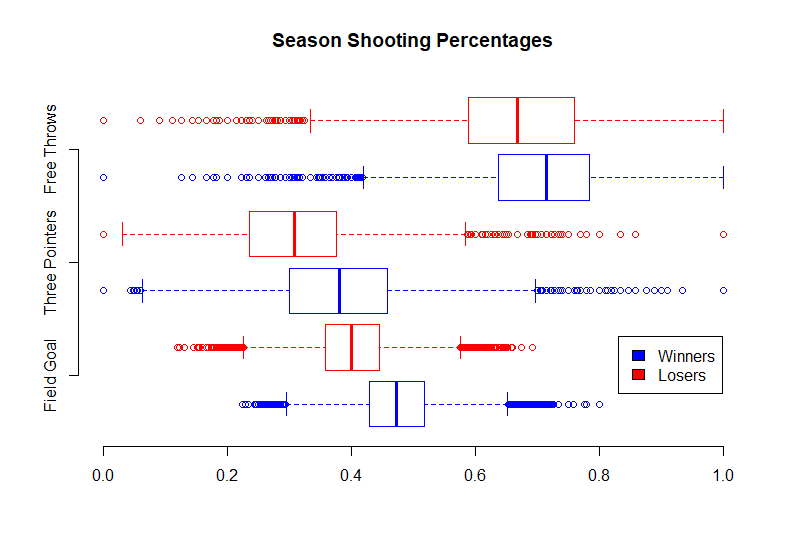
\includegraphics[scale=.5]{SeasonShotPercent.png}
\end{figure}
This figure visualizes the differences that exist, on average, in winning and losing teams' shot percentages. There are a large number of outliers in this plot, which should be noted for future analysis. It is also hard to tell which shots look to be more influential in the winning of a game because the data is so wide-spread.
\subsection*{Tournament Data}
Much the same as when we worked with the regular season data, we analyzed the tournament data at first on a more basic level of winning teams versus losing teams. Much of the data that we had for tournaments was centered on the teams' abilities to score. We analyzed their shooting percentages during the tournaments and compared average winning teams to average losing teams.
\begin{figure}[H]
	\centering
	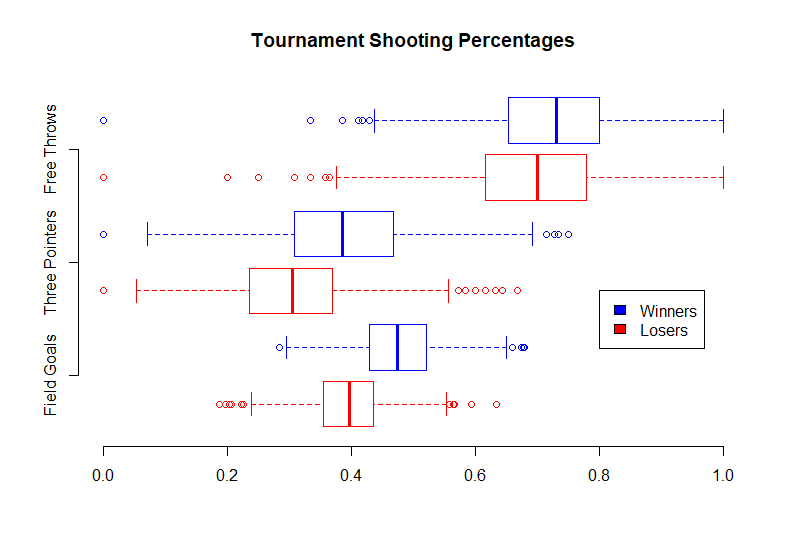
\includegraphics[scale=.5]{TourneyShotPercent.png}
\end{figure}
As the above figure illustrates, winning teams, on average, have higher shooting percentages in all categories. It is essential to note how large the differences may be. From this data we can start to decide which types of shots are the most important to tournament success.
\subsection*{History of Success}
As a result of looking at our data, and through our own personal knowledge of the sport, we decided it was fitting to look into each team's history of success in the tournament and how often they had been seeded near the top.
\begin{figure}[H]
	\centering
	\includegraphics[scale=.5]{overLeaders.pdf}
\end{figure}
The above figure maps how often teams have been seeded among the top four, for any region in the tournament. Teams that have been successful in the past are more likely to be seeded near the top again in the future, as is pictured above. The teams near the top of this chart are those that are commonly discussed amongst basketball fans. They are teams that come from schools that are known for basketball, and they likely draw in more talented players as a result of their reputation, helping them further develop their program.

We continue this analysis of History of Success by looking at teams that are all-around leaders in past tournaments. We look at each team's past appearances in the tournament to compare them to each other.
\begin{figure}[H]
	\centering
	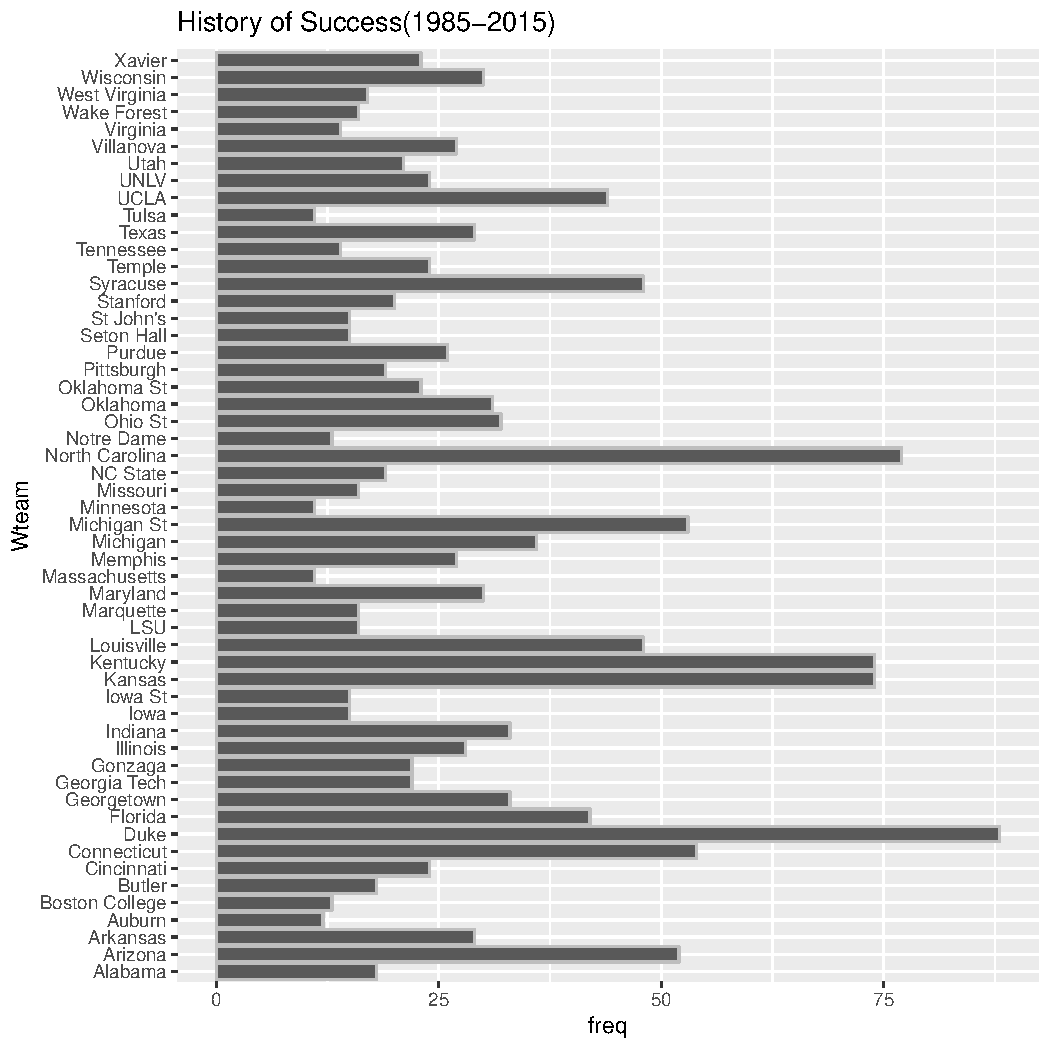
\includegraphics[scale=.5]{HistOfSuccess2.pdf}
\end{figure}
The figure above shows some of the teams with the most appearances in the March Madness tournament. Higher frequency logically relates to a better team, and this data allows us to see which teams are consistently present and performing in the tournament.

\section*{Initial Model}
	\[
Y_{daynum} = \beta_0 + \beta_{conf} + \beta_{fgp} +\beta_{tpp} + \beta_{ass} + \beta_{rb} + \beta_{app} + \epsilon
\]
Our original model contained all of the predictors that we felt would be the most important moving forward. These predictors and subscripts are outlined below:
	\begin{itemize}
	\item The response variable, {\textit{daynum}}, signifies what day of the year the last game is played for each team. This is a good measure of two things: If a team makes the tournament and how far that team advances.
	\item 	{\textit{conf:}} the conference the team plays in - different conferences have vastly different quality of teams
	\item 	{\textit{fgp:}} refers to field goal percentage
	\item 	{\textit{tpp:}} three point shooting percentage
	\item 	{\textit{ass:}} assists
	\item 	{\textit{rb:}} rebounds
	\item 	{\textit{app:}} prior tournament success - indicated by number of previous appearances in the tournament
	\end{itemize}
Seed is not included because seeding is almost entirely determined by conference and record. Record is left out because it is in large part determined by a teams statistics, which we have included in the model.
\section*{Processing}
In working with our data to develop a model, we realized that there may be a better way to interpret it. We also ran into problems with some predictors and variables because they were quite difficult to quantify or compare.

We found that {\textit{daynum}} may not be the best measure of a team's success in the tournament because the respective games of a tournament are played on slightly different days each year. This means that the team who won the tournament in 2003 could have a higher daynum than the team who won the tournament in 2004, automatically ranking the 2003 team higher, although they played and won the same number of games.

We also found that {\textit{conf}} was difficult to quantify because while some conferences are undoubtedly better than others, it is not up to our judgment as to decide how much better they are and which conferences deserve to be credited as the best.
\subsection*{Data Plumbing}
\subsection*{Data Reconstruction}
\section*{Full Model}
	\[
Y_{GP_{year}} = \beta_0 + \beta_{avgScore} + \beta_{avgASS} +\beta_{avgFT} + \beta_{avgPF} + \beta_{avgTP} + \beta_{avgRB} + \beta_{avgTO}
\] 
\[
+ \beta_{avgSTL} +\beta_{avgBL} + \beta_{GP_{year-1}}+ \epsilon
\]
We fit a full model with all of the possible predictors that we pulled from the data. The full list of predictors includes:
	\begin{itemize}
	\item 	{$GP_{year}$:} number of games the team plays in the tournament in a given year
	\item 	{\textit{avgScore:}} average score per team per game in regular season
	\item 	{\textit{avgASS:}} average assists per team per game in regular season
	\item 	{\textit{avgFT:}} average free throws per team per game in regular season
	\item 	{\textit{avgPF:}} average personal fouls per team per game in regular season
	\item 	{\textit{avgTP:}} average three point shots made per team per game in regular season
	\item 	{\textit{avgRB:}} average total rebounds per team per game in regular season
	\item 	{\textit{avgTO:}} average turnovers per team per game in regular season
	\item 	{\textit{avgSTL:}} average steals per team per game in regular season
	\item 	{\textit{avgBL:}} average blocks per team per game in regular season
	\item 	{$GP_{year-1}$:} number of games the team plays in the tournament in the prior year
	\end{itemize}
We formed this model for each year from 2003 to 2015 because those are the years that we have the most data for, and we seek out the model with the highest $R^{2}$ value because it accounts for the most variation in the response. The coefficients and summary of some of the models are shown below:
\begin{verbatim}
Insert clippings from R code
\end{verbatim}
\section*{Full Model Analysis}
\section*{Final Model}
	\[
Y_{GP_{year}}^{-0.5} = \beta_0 + \beta_{avgASS} +\beta_{avgFT} + \beta_{avgPF} + \beta_{avgFG} + \beta_{avgTO} + \beta_{GP_{year-1}}+ \epsilon 
\]
\section*{Final Model Analysis}
\section*{Predictions}
\section*{Further Research}
\section*{Appendix}

\end{document}
